\lstset{language={Python2}}

\title{ALPSチュートリアル: ALPS Python入門}

\begin{document}

\begin{frame}
 \titlepage
\end{frame}

\section*{Outline}
\begin{frame}
 \tableofcontents
\end{frame}

\section{ALPS python}

\subsection*{\redm\whiteb\greenb}
\begin{frame}[t,fragile]
 \frametitle{Launching Python}
 \begin{itemize}
 \item \alert{ALPS を Python のモジュールとして利用することが可能.}

 \item MateriApps LIVE! では標準でパスが設定済. 普通にpython (あるいはipython)を実行するだけでALPS Pythonが利用可能.

 \item その他の環境では、ALPSをインストールした場合に同時にインストールされるalpsvars.shファイルを読み込んだ上で、python (あるいはipython)を実行.
\begin{lstlisting}
$ source /somewhere/alpsvars.sh
$ python
\end{lstlisting}
\end{itemize}
\end{frame}

\section{パラメータの準備}

\subsection*{\redm\whiteb\greenb}
\begin{frame}[t,fragile]
 \frametitle{Importing ALPS modules}

\begin{itemize}
 \item ALPS Python を Python のインタープリタから利用してみよう.
       (できれば iPython を使った方がよい)
       
\begin{lstlisting}
$ ipython
>>> import pyalps
\end{lstlisting}
       なにもエラーが出なければこれで準備終了.


 \item iPython の場合 Tab 補完で pyalps のモジュールや関数などが列挙できる

\begin{lstlisting}
>>> al.[ここで Tab]
Display all 102 possibilities? (y or n)
al.CycleColors   
al.CycleMarkers  
...            
\end{lstlisting}
\end{itemize}
\end{frame}

\subsection*{\redm\whiteb\greenb}
\begin{frame}[t,fragile]
\frametitle{Preparing parameter}

1回のシミュレーションに必要なパラメータセットを辞書型で与える


温度 $T = 1.5, 2, 2.5$ と変化させ 3 回のシミュレーションを行う例

\begin{lstlisting}
>>> parms = []
>>> for t in [1.5,2,2.5]:
...    parms.append({'LATTICE': "square lattice", 
...    'T': t,  'J': 1 ,
...    'THERMALIZATION': 1000, 'SWEEPS': 100000,
...    'UPDATE': "cluster", 'MODEL': "Ising",
...    'L': 8})
>>>
\end{lstlisting}

辞書型の要素を 3 つ持つリスト params ができる
% [ {'LATTICE': "square lattice", 'T': t,  'J': 1 ,'THERMALIZATION': 1000, 'SWEEPS': 100000,'UPDATE': "cluster", 'MODEL': "Ising", 'L': 8} for t in [1.5,2,2.5]]
\end{frame}

\subsection*{\redm\whiteb\greenb}
\begin{frame}[t,fragile]
\frametitle{Preparing input XML files}
パラメータから XML 形式の入力ファイルを作成する
\begin{lstlisting}
>>> mkdir sim         # シミュレーション用のディレクトリを作成し
>>> cd sim            # そこへ移動する
>>> input_file = pyalps.writeInputFiles('parm1',parms)
>>> print input_file  # 入力ファイル名が返されている
parm1.in.xml
>>> ls                # 作成されたファイルを確かめる.
ALPS.xsl parm1.in.xml parm1.task1.in.xml parm1.task2.in.xml parm1.task3.in.xml
\end{lstlisting}
\begin{itemize}
 \item parm1.in.xml はシミュレーション全体の入力ファイル
 \item parm1.task\# .in.xml は各タスク毎の入力ファイル
\end{itemize}

\end{frame}

\section{シミュレーションの実行}

\subsection*{\redm\whiteb\greenb}
\begin{frame}[t,fragile]
\frametitle{Running simulation on serial machine}
\begin{lstlisting}
>>> pyalps.runApplication('spinmc', input_file,Tmin=5,writexml=True)
spinmc parm1.in.xml --Tmin 5 --write-xml
Generic classical Monte Carlo program using local or cluster updates
...
Checkpointing Simulation 3
Finished with everything.
(0, 'parm1.out.xml')
\end{lstlisting}
\begin{itemize}
\item 実行が終了すると parm1.out.xml, parm1.task1.out.h5, $\cdots$ といったファイルが出力されている
\end{itemize}
\end{frame}

\subsection*{\redm\whitem\greenb}
\begin{frame}[t,fragile]
\frametitle{Running simulation on parallel machine}
\begin{lstlisting}
>>> pyalps.runApplication('spinmc',input_file,Tmin=5,writexml=True,MPI=4)
\end{lstlisting}
\begin{itemize}
\item MPI=4 で MPI プロセス 4 並列でシミュレーションを実行することを指示
\end{itemize}
\end{frame}

\section{実行結果の読み込み}

\subsection*{\redm\whiteb\greenb}
\begin{frame}[t,fragile]
 \frametitle{Getting result files}
\begin{lstlisting}
>>> result_files = pyalps.getResultFiles(prefix='parm1')
>>> print result_files
['./parm1.task2.out.xml', './parm1.task3.out.xml', './parm1.task1.out.xml']
\end{lstlisting}
 \begin{itemize}
  \item カレントディレクトリ内からプレフィックスが 'parm1' のファイルを正規表現によるパターンマッチで探してファイル名を出力
  \item result\_files はファイル名のリスト.
 \end{itemize}
\end{frame}

\subsection*{\redm\whiteb\greenb}
\begin{frame}[t,fragile]
\frametitle{Loading results}
指定したファイル名のリストから,指定した物理量(複数可)を取り出す
\begin{lstlisting}
>>> data = pyalps.loadMeasurements(result_files,['|Magnetization|','Magnetization^2'])
>>> data[0]  # data の中身をみてみる
[x=[0]
y=[0.083339021352 +/- 0.00038780838614]
props={'observable': '|Magnetization|', 'THERMALIZATION': 10000.0, 'J': -1.0, ...}, 
x=[0]
y=[0.00816759554762 +/- 7.41432666026e-05]
props={'observable': 'Magnetization^2', 'THERMALIZATION': 10000.0, 'J': -1.0, ...}]
\end{lstlisting}
\end{frame}

\subsection*{\redm\whiteb\greenb}
\begin{frame}[t,fragile]
\frametitle{データの構造}
シミュレーション結果を表すクラス
\begin{itemize}
\item \textbf{DataSet}: class 名
  \begin{itemize}
  \item x: plot 用のインデックス (最初はデフォルト値 0 が入っている)
  \item y: 物理量の平均値および標準誤差
  \item props: 物理量名およびパラメータなどが Python の辞書形式で入っている
  \end{itemize}
\end{itemize}

\begin{lstlisting}
# 物理量の平均値と標準誤差を取り出してみる
>>> data[0][0].y
array([0.083339021352 +/- 0.00038780838614], dtype=object)
>>> data[0][0].y.mean
0.08333902135203504
>>> data[0][0].y.error
0.00038780838614
\end{lstlisting}
\end{frame}

\section{結果のプロット}

\subsection*{\redm\whiteb\greenb}
\begin{frame}[t,fragile]
\frametitle{Plotting the results}
\begin{lstlisting}
>>> plotdata = pyalps.collectXY(data,'T','|Magnetization|')
>>> plotdata[0].x
array([ 1.5,  2. ,  2.5])
>>> plotdata[0].y
array([0.986621683313 +/- 5.59763992999e-05,
       0.911889051072 +/- 0.000288443276697,
       0.605402476752 +/- 0.0013356753695], dtype=object)
>>> plotdata[0].props
{'observable': '|Magnetization|', '...
\end{lstlisting}
\begin{itemize}
\item data から pyalps.collectXY により x 軸として 'T', y 軸として '$|$Magnetization$|$' を取り出している
\end{itemize}
\end{frame}

\subsection*{\redm\whiteb\greenb}
\begin{frame}[t,fragile]
\frametitle{Plotting in Python using matplotlib}
\begin{lstlisting}
>>> pyalps.plot.plot(plotdata) # データをプロット.
[<matplotlib.lines.Line2D at 0x109425dd0>]
>>> plt.xlim(0,3)             # x 軸の範囲を設定
>>> plt.ylim(0,1)             # y 軸の範囲を設定
>>> plt.title('Ising model')  # 図のタイトル
>>> plt.savefig('ising.pdf')  # ファイルへ出力
>>> plt.show()                # X11 などで画面に表示
\end{lstlisting}
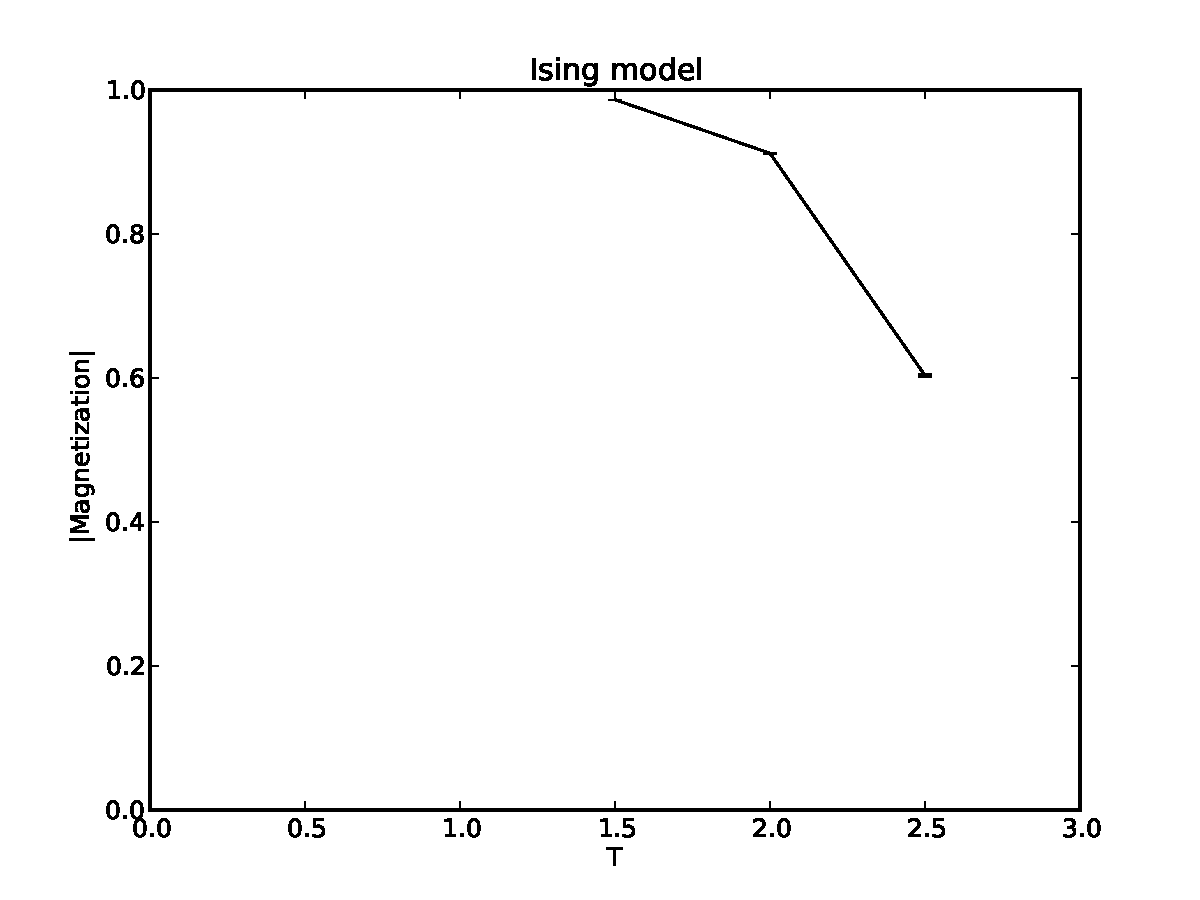
\includegraphics[scale=0.2]{ising.pdf}
\end{frame}

\subsection*{\redm\whiteb\greenb}
\begin{frame}[t,fragile]
\frametitle{Converting to other formats}
ほかのデータフォーマットに変換できる
\begin{lstlisting}
>>> print pyalps.plot.convertToText(plotdata)
>>> print pyalps.plot.makeGnuplotPlot(plotdata)
>>> print pyalps.plot.makeGracePlot(plotdata)
\end{lstlisting}

text 形式の出力例
\begin{lstlisting}
# 
# X: T
# Y: |Magnetization|
1.5	0.986496240665 +/- 2.82049446481e-05
2.0	0.912126100521 +/- 0.000350201474667
2.5	0.603552651599 +/- 0.00146115425377
\end{lstlisting}
\end{frame}

\section{結果の評価}

\subsection*{\redm\whiteb\greenb}
\begin{frame}[t,fragile]
\frametitle{Example of evaluating data}
binder 比 $<m^2>/<|m|>^2$ の計算をしてみる
\begin{lstlisting}
>>> binder = pyalps.DataSet()
>>> binder.props = pyalps.dict_intersect([d[0].props for d in data])
>>> binder.x = [d[0].props['T'] for d in data]
>>> binder.y = [d[1].y[0]/(d[0].y[0]*d[0].y[0]) for d in data]
>>> print binder
\end{lstlisting}
\begin{itemize}
\item 空のデータセットを作る
\item 複数の辞書から key:val ともに一致する項目を抜き出す
\item データから x 軸となる 'T' の数列をとりだす.
\item $d[0]$ から $m^2$, $d[1]$ から $|m|$ を取り出して binder 比を計算
\end{itemize}
\end{frame}

\end{document}
